% =============================================================================
% Archi --- CHEP 2026 paper, main orchestrator file.
%
% Read paper/style-notes.md before drafting any prose.
%
% Layout: one .tex file per section. This file is the orchestrator only ---
% no body content lives here.
%
% Build: pdflatex main && bibtex main && pdflatex main && pdflatex main
% =============================================================================

\documentclass[twocolumn]{webofc}
% webofc loads: amsmath, amssymb, graphicx, url, fontenc, inputenc,
% babel (english), eurosym, calc, fancyhdr, cuted, geometry.
\usepackage{booktabs}
\usepackage{hyperref}
\usepackage{arydshln}
\usepackage{tikz}
\usetikzlibrary{positioning, arrows.meta, fit, calc}
\usepackage{xcolor}
\definecolor{docgreen}{HTML}{2E7D5A}
\definecolor{docfill}{HTML}{E6F2EA}
\definecolor{liveorange}{HTML}{C75B25}
\definecolor{livefill}{HTML}{FBE6D8}
\definecolor{agentblue}{HTML}{0072B2}
\definecolor{agentfill}{HTML}{DCEAF8}

% \todocell --- visible placeholder for table cells whose values come from
% in-flight benchmark runs. Renders as \textit{TBD} so it is unmistakable in
% the PDF and greppable in source.
\newcommand{\todocell}{\textit{TBD}}

\title{Archi: An Agent for CMS Computing Operations}
\titlerunning{Archi}
\authorrunning{Archi authors}
\author{%
  \firstname{TBD} \lastname{TBD}\inst{1}
}
\institute{%
  TBD --- co-author affiliations populated before submission.
}

\begin{document}

\abstract{%
Archi is the operator chat agent deployed for CMS Computing
Operations (CompOps) since February 2026. CompOps spans three
activities: Tier-0 reconstruction with dual-tape archival,
Production \& Reprocessing of Monte Carlo and data-reprocessing
campaigns through the Workflow Management system, and
Rucio-based Data Management across more than sixty Tier-1 and
Tier-2 WLCG sites. Operators field questions about all three from CMS TWiki
runbooks, the CompOps Jira ticket history, and the live MonIT
operational-state index. Archi pairs hybrid retrieval over the
TWiki and Jira with live MonIT queries against Rucio and HTCondor
in a ReAct loop, surfacing tool traces for operator audit.
We sample a 260-question evaluation set from six weeks of
production operator traffic (144 answerable from documentation
alone, 116 requiring a live tool call) and benchmark four
pipeline layers (bare LLM, RAG, agent without live tools, full
agent) on three open-weight models against the GPT-5.3
production answers re-scored on the same rubric. Each layer
earns a measurable lift: bare LLM 2.86, RAG 3.97 (+1.1), agent
without live tools 4.22 (+0.25), and live MonIT calls add
0.19 more points on the 20\% of operator traffic that needs
operational state. On the largest open-weight model the full
agent reaches $4.22 \pm 0.06$ against the GPT-5.3 production
reference's $4.08 \pm 0.08$ under \texttt{glm-5.1}. A four-judge
LLM ensemble on a 53-question subset preserves the pipeline
ordering, and a parallel human evaluation by a panel of five
CMS Computing Operations domain experts is in progress.
}

\maketitle
\section{Introduction}
\label{sec:introduction}

CMS Computing Operations
(CompOps)~\cite{cms_computing_tdr,cms_compops} turns raw CMS
detector output into usable scientific data through three
activities (Section~\ref{sec:workload}): Tier-0 repacks the
detector stream, archives two tape copies, and runs express and
prompt reconstruction; Production \& Reprocessing drives Monte
Carlo and reprocessing campaigns through the CMS Workflow
Management system; and Data
Management~\cite{cms_dm2025} executes transfers and placement
across more than sixty Tier-1 and Tier-2 WLCG sites with
Rucio~\cite{rucio2014,cms_rucio2020}.
Day-to-day, CompOps operators run workflows, triage tickets,
watch live operational state (the MonIT index, surfaced through
OpenSearch and Grafana), conduct root-cause analysis, and onboard
new team members; their support is fragmented across the CMS
TWiki, the CompOps Jira projects, MonIT, and Mattermost channels,
and resolving a stalled transfer requires the runbook entry, the
current MonIT counters, and the ticket history of past stalls on
the same link.

Archi is an operator chat agent deployed for CompOps since 16
February 2026. Archi combines retrieval over the CMS TWiki and
CompOps Jira with live MonIT calls and surfaces the tool trace
for operator audit. The production pipeline uses GPT-5; to
evaluate local-weight alternatives we sample a 260-question
subset from the recorded conversations after deduplication and
filtering (Section~\ref{sec:question_patterns}; 144 answerable
from documentation alone, 116 requiring a live tool call) and
re-score the GPT-5.3 production answers on the same rubric as
the GPT-5.3 reference.

Each pipeline layer earns a measurable lift on the rubric. On
the largest open-weight model the bare LLM scores 2.86, the
RAG control 3.97, the agent without live tools 4.22, and the
full agent 4.22 in aggregate with $+0.19$ on the 20\% of
operator traffic that needs operational state. The full agent
at $4.22 \pm 0.06$ matches the GPT-5.3 production reference at
$4.08 \pm 0.08$ under the same judge.
Section~\ref{sec:agent} describes the agent and its tool
surface, Section~\ref{sec:evaluation} the four-layer rubric
evaluation and a four-judge replication, and
Section~\ref{sec:discussion} the trade-offs the agent loop
carries.

\section{The CMS Computing Operations Workload}
\label{sec:workload}

CompOps operations cover three computing activities and pull
operator support from four information sources.
Section~\ref{sec:compops_domain} describes the activities and
the source layout; Section~\ref{sec:question_patterns}
introduces the 260-question evaluation set extracted from
production traffic; Section~\ref{sec:workflows} traces three
recurring workflows that exercise the tool families.

\subsection{Computing Operations at CMS}
\label{sec:compops_domain}

The three activities of Section~\ref{sec:introduction} (Tier-0,
P\&R, Data Management) all emit operational state into a shared
layer: workflow state, transfer rates, job-failure counts, and
site-readiness metrics are aggregated into MonIT and surfaced
through OpenSearch and Grafana~\cite{cms_monit}. CompOps
responsibilities split across operators, workflow managers, and
campaign managers, working in shifts across CERN, FNAL, INFN, and
other collaboration centres with daily handover on Mattermost and
ticket-driven escalation to on-call experts. Recurring questions in operator traffic include: where a
transfer is stuck, why a workflow has resubmitted five times,
which site is in downtime, what the runbook says about an error
code, whether a given Jira ticket is already known, and which
procedure a new team member should follow.

Four sources cover the answer space: the CMS TWiki holds the
documented procedures; the Jira project holds the ticket history
with assignees and resolutions; MonIT holds the time-series of
operational counters; and the \texttt{cms-comp-ops} Mattermost
channel holds the unwritten context not yet in a runbook.
Diagnosing a stalled transfer typically starts from the runbook
entry, requires the current MonIT counters and the site's
readiness status, and ends with the Jira-ticket history of past
stalls on that link.

\subsection{Operator Question Patterns}
\label{sec:question_patterns}

The 260-question evaluation set is sampled from the deployed
assistant's traffic between 16 February and 30 March 2026, after
deduplication and filtering of non-English messages, empty turns,
and development-team conversations; it exposes three patterns
relevant to the agent design.
First, operator questions split roughly evenly between
documentation and live state: 144 of 260 questions can be answered
from the documented procedure alone, and 116 require a live tool
call against Jira or MonIT.
Second, 108 of 260 questions (42\%) are part of a multi-turn
conversation: a follow-up such as ``which site was that?''
resolves only against the preceding turns.
Third, 55 of 260 questions (21\%) refer to time-sensitive
operational state, where an answer correct on Monday is wrong on
Friday.

We labelled each question with one of six categories chosen to
match how operators phrase their questions rather than how the
agent answers them.
The labels are assigned by a deterministic rule-based classifier
that walks each question through a fixed priority order: log-trace
dumps fall to \textit{debugging}; questions containing a CMS Jira
ticket reference (\texttt{CMSPROD-}, \texttt{CMSTRANSF-},
\texttt{CMSCOMPPR-}, $\dots$) fall to \textit{jira\_investigation};
questions about counts in a recent window fall to
\textit{data\_query}; imperative ``how do I'' patterns fall to
\textit{procedural}; ``summarize'' and ``explain'' patterns fall
to \textit{exploratory}; everything remaining is
\textit{factual\_lookup}.
We chose rule-based labelling over an LLM-assigned scheme because
the categories are defined by surface-form features and the
labelling has to be reproducible across curation passes.

The category distribution reflects the steady-state CompOps
workload during the six-week sampling window.
Factual lookups (76 questions, 29\%) are the largest single
category: examples include which storage element backs a given
site, what Rucio rule applies to a particular dataset, or what a
particular configuration value means.
Data queries (52 questions, 20\%) and Jira investigations (39
questions, 15\%) together account for the live-access half of the
workload: both require a tool call, but data queries hit MonIT
counters while Jira investigations hit the ticket history.
Procedural and exploratory questions (34 each, 13\%) follow.
Debugging questions (25, 10\%) are the smallest category and
cover cases where the operator dumps a full log into the chat.

The doc-answerable / live-access split follows the categories
deterministically: factual, procedural, and exploratory questions
are doc-answerable; data, Jira, and debugging questions require a
live tool call.
The agent has to handle both halves; the controls without
live-tool access (Section~\ref{sec:evaluation}) can only handle
the doc-answerable half by construction.
Figure~\ref{fig:workload} shows the breakdown.

\begin{figure}[htbp]
\centering
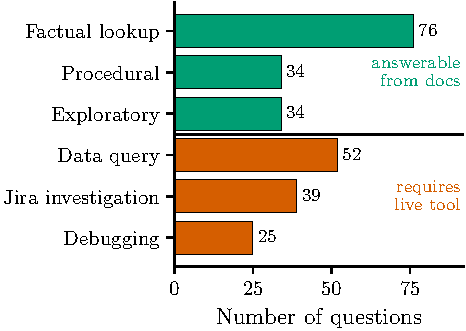
\includegraphics[width=\columnwidth]{figs/fig_workload.pdf}
\caption{Operator questions split roughly evenly between
documentation-answerable (144, green) and live-tool-required
(116, red) categories. The 260-question evaluation set by
category.}
\label{fig:workload}
\end{figure}

\subsection{Common operator workflows}
\label{sec:workflows}

Three workflows distilled from the recorded operator traffic
illustrate how the tool families combine.

\emph{Stalled transfer triage.} An operator sees a transfer to
a Tier-2 site failing and asks Archi why. The agent issues parallel
tool calls: an HTCondor MonIT aggregation over recent transfer
events, a CompOps Jira retrieval for tickets referencing the site
or source, and a CMS TWiki retrieval over the transfer-recovery
runbook. It returns the site-readiness status, the most recent
matching ticket, and the runbook section for the failure mode.

\emph{Workflow resubmission diagnosis.} For a workflow that has
resubmitted five times, the agent aggregates HTCondor MonIT
failure codes, retrieves the workflow's Jira ticket plus similar
past resubmissions, and looks up the resubmission runbook;
returns the failure pattern, prior resolutions, and recommended
action.

\emph{Procedure lookup.} For a stuck Tier-0 stream, the agent
retrieves the Tier-0 runbook from the TWiki and recent Tier-0
tickets from Jira; returns the recovery procedure and the most
recent tickets touching it.

\section{The Archi Agent}
\label{sec:agent}

Archi is implemented as an open-source Python framework
configured per deployment; this section describes the CompOps
configuration. Section~\ref{sec:components} covers the three
top-level components, Section~\ref{sec:pipelines} the agent
pipeline and the controls evaluated against it,
Section~\ref{sec:tools} the tool catalogue, and
Section~\ref{sec:deployment} the production rollout.

\subsection{Components}
\label{sec:components}

The framework decomposes into three components: a data manager
that ingests and indexes documentation sources, a pipeline layer
that the chat service routes user questions through, and a chat
interface. Figure~\ref{fig:architecture} shows the top-level
dataflow.

\begin{figure}[htbp]
\centering
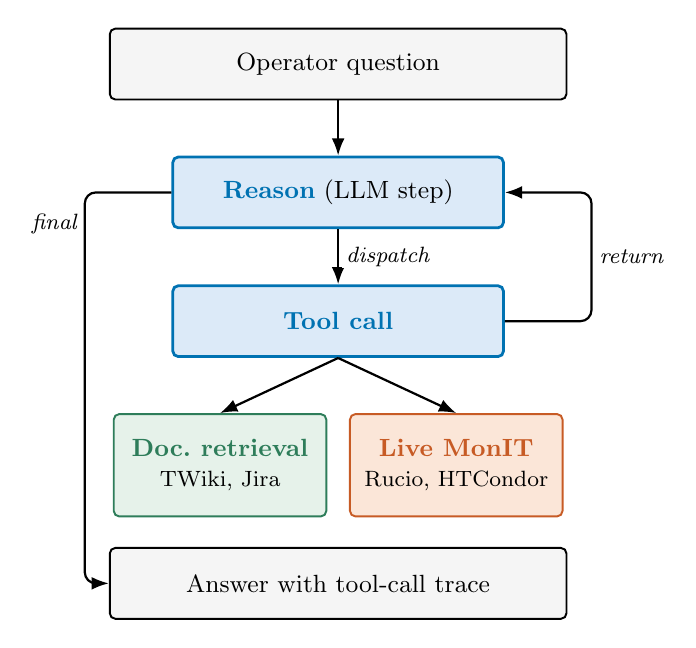
\begin{tikzpicture}[
    >={Latex[length=2.2mm]},
    every node/.style={font=\small},
    node distance=7mm,
    box/.style={
        rectangle, rounded corners=2pt, draw, line width=0.7pt,
        inner sep=3pt, align=center, minimum height=9mm,
    },
    iobox/.style={box, fill=gray!8, minimum width=58mm},
    rxn/.style={box, fill=agentfill, draw=agentblue, line width=1.0pt,
        minimum width=42mm},
    docbox/.style={box, fill=docfill, draw=docgreen, line width=0.7pt,
        minimum width=27mm, minimum height=13mm},
    livebox/.style={box, fill=livefill, draw=liveorange, line width=0.7pt,
        minimum width=27mm, minimum height=13mm},
    arrlbl/.style={font=\footnotesize\itshape, inner sep=1.5pt,
        fill=white, inner ysep=0.5pt}
]

% Top: question
\node[iobox] (q) {Operator question};

% ReAct loop core
\node[rxn, below=of q] (reason)
    {\textcolor{agentblue}{\textbf{Reason}} (LLM step)};
\node[rxn, below=of reason] (tool)
    {\textcolor{agentblue}{\textbf{Tool call}}};

% Tool families
\node[docbox, below=of tool, xshift=-15mm] (docs)
    {\textcolor{docgreen}{\textbf{Doc.\ retrieval}}\\
     \footnotesize TWiki, Jira};
\node[livebox, below=of tool, xshift=15mm] (live)
    {\textcolor{liveorange}{\textbf{Live MonIT}}\\
     \footnotesize Rucio, HTCondor};

% Final answer below, centered under the loop
\node[iobox, below=24mm of tool] (out)
    {Answer with tool-call trace};

% --- Forward flow ---
\draw[->, line width=0.8pt] (q.south) -- (reason.north);
\draw[->, line width=0.8pt] (reason.south) -- (tool.north)
    node[arrlbl, midway, right=1pt] {dispatch};
\draw[->, line width=0.8pt] (tool.south) -- (docs.north);
\draw[->, line width=0.8pt] (tool.south) -- (live.north);

% --- Loop back: tool return on the right ---
\draw[->, line width=0.8pt, rounded corners=4pt]
    (tool.east) -- ++(11mm,0) |- (reason.east)
    node[arrlbl, pos=0.25, right=1pt] {return};

% --- Final exit: reason directly emits the answer (curves down on the left) ---
\draw[->, line width=0.8pt, rounded corners=4pt]
    (reason.west) -- ++(-11mm,0) |- (out.west)
    node[arrlbl, pos=0.04, left=1pt] {final};

\end{tikzpicture}
\caption{Archi's ReAct loop. Each iteration the
\textsc{Reason} step dispatches a \textsc{Tool call} (either
documentation retrieval or live MonIT), and the tool return
becomes the next reason input. When \textsc{Reason} decides no
further tools are needed it emits the answer with its tool-call
trace.}
\label{fig:architecture}
\end{figure}

The data manager ingests web pages, git repositories, local
files, and Jira projects into a PostgreSQL \texttt{pgvector}
index of chunked passages embedded with
\texttt{sentence-transformers/all-MiniLM-L6-v2}~\cite{reimers2019sbert}.
For the CompOps deployment the sources are the CMS TWiki, a
curated list of public CMS documentation repositories, and seven
CompOps Jira projects (\texttt{CMSPROD}, \texttt{CMSTRANSF},
\texttt{CMSDM}, \texttt{CMSTZ}, \texttt{PRCAMPAIGNS},
\texttt{CMSMONIT}, \texttt{CMSVOC}); ticket text is anonymised at
ingest.

A pipeline takes a question, the prior conversation, and the
deployment configuration, and returns an answer with the
documents and tool calls that supported it. Pipelines are
declared in YAML and selected per deployment; the pipelines
compared in Section~\ref{sec:evaluation} differ on two axes:
whether they retrieve from the documentation store and whether
they call live MonIT.

\subsection{The CompOps Agent}
\label{sec:pipelines}

The deployed assistant runs an agent built on the ReAct pattern
\cite{yao2023react} using the LangGraph state-graph framework
\cite{langgraph}.
The graph alternates a reasoning step (which emits a textual
trace) with a tool-call step (which invokes either a
documentation-retrieval tool or a live MonIT query); when the
reasoning step decides no further tools are needed, it emits the
final answer with the accumulated tool-call trace.
The system prompt steers the agent toward parallel exploratory
tool calls, aggregation queries when counting, and fetch-by-ID
fallback when a search returns only summaries. It also forbids
asking the operator for clarification, requiring a best-guess
answer with explicit refusal when live state is unreachable.

Two control pipelines and one ablation are summarised in
Table~\ref{tab:pipeline_summary}. The bare-LLM control sends the
question and conversation history directly to the language model;
the RAG control retrieves the top-eight passages from the
documentation store using a hybrid BM25-plus-vector retriever and
conditions on them~\cite{lewis2020rag}; the \emph{agent (no live
tools)} ablation runs the agent with the live MonIT tools removed
while retaining documentation retrieval, isolating the
contribution of live MonIT relative to the full agent and the
contribution of the agent loop relative to RAG.

\begin{table}[htbp]
\centering
\caption{The four pipelines compared in this paper, including a
no-live-tools ablation of the agent. Documentation refers to the
hybrid retriever over the CMS TWiki and ingested Jira tickets;
MonIT refers to live OpenSearch queries against the Rucio and
HTCondor monitoring indices.}
\label{tab:pipeline_summary}
\begin{tabular}{lcc}
\toprule
\textbf{Pipeline} & \textbf{Documentation} & \textbf{Live MonIT} \\
\midrule
Bare LLM               & no  & no  \\
RAG                    & yes & no  \\
Agent (no live tools)  & yes & no  \\
Agent                  & yes & yes \\
\bottomrule
\end{tabular}
\end{table}

\subsection{Tools}
\label{sec:tools}

The agent has access to three tool families, listed in
Table~\ref{tab:tool_catalogue}: documentation retrieval, the
Rucio data-management MonIT index, and the
HTCondor~\cite{htcondor2005} jobs MonIT index. Each MonIT family
exposes search, aggregation, and fetch variants; the documentation
family exposes hybrid BM25-plus-vector search, metadata-index
browse, and fetch-by-ID. MonIT tools authenticate against the
central CERN Grafana-OpenSearch endpoint with bearer tokens; every
tool call is recorded in the trace surfaced to the operator.

\begin{table}[htbp]
\centering
\caption{Tools exposed to the agent. Each family supports a
search, an aggregation, and a fetch-by-ID variant against its
backend.}
\label{tab:tool_catalogue}
\begin{tabular}{@{}lp{0.55\columnwidth}@{}}
\toprule
\textbf{Family} & \textbf{Backend} \\
\midrule
Documentation  & \texttt{pgvector} over CMS TWiki and Jira tickets \\
Rucio MonIT    & WLCG OpenSearch, Rucio events \\
HTCondor MonIT & WLCG OpenSearch, HTCondor jobs \\
\bottomrule
\end{tabular}
\end{table}

\subsection{Production Deployment}
\label{sec:deployment}

Archi has run as the CMS CompOps operator chat assistant since
February 2026 on shared CMS infrastructure at CERN, serving the
operations team, on-call experts, and contributors debugging
production workflows. Operators interact through a web chat interface that
maintains turn-by-turn conversation history, lists source
documents per response, and exposes the agent's tool-call trace.
The deployed pipeline runs on GPT-5; the evaluation in
Section~\ref{sec:evaluation} re-scores those production answers
on the same rubric and benchmarks local-weight alternatives
against them.

\section{Evaluation}
\label{sec:evaluation}

The evaluation asks four questions of the deployment: does an
LLM alone suffice for CompOps operator questions? Does a RAG
pipeline over the documented corpus suffice? Does the agent
loop earn its keep over single-shot RAG? Do live MonIT tool
calls earn their cost over a doc-only agent?
Section~\ref{sec:eval_methodology} states the configurations,
models, and infrastructure for the two experimental tracks
(260-question single-judge matrix on local Ollama, 53-question
multi-judge subset on OpenRouter).
Section~\ref{sec:eval_lifts} walks the four-step lift from a
bare LLM (\textbf{2.86}) to the full agent (\textbf{4.22})
under \texttt{glm-5.1} on the 260-question set.
Section~\ref{sec:eval_costs} surfaces the two costs the agent
loop carries.
Section~\ref{sec:eval_ensemble} replicates the ordering under a
four-judge ensemble on a 53-question subset.
Section~\ref{sec:eval_human_53} reports the human evaluation
panel.

\subsection{Configurations, models, and infrastructure}
\label{sec:eval_methodology}

Two experimental tracks share the same rubric and pipeline
definitions but differ in scale, judge protocol, and model
selection.

\paragraph{260-question matrix on local Ollama.}
The four pipelines of Section~\ref{sec:pipelines} (the bare-LLM
control, the RAG control, the agent without live operational
tools, and the agent) run on three locally-served open-weight
models: \texttt{gemma4-26b}~\cite{gemma4card}, a Google
mixture-of-experts (MoE) with 26\,B total and 4\,B active
parameters; \texttt{qwen3.5-27b}~\cite{qwen3report}, a 27\,B
dense model from Alibaba; and
\texttt{qwen3.5-122b-a10b}~\cite{qwen3report}, a 122\,B MoE
with 10\,B active per token. Each (pipeline, model) combination
runs with the model's extended-thinking mode (the model emits a
chain-of-thought trace before its answer) enabled and,
separately, disabled. All models in this track are served
through Ollama~\cite{ollama} on a CMS-internal node with four
NVIDIA Tesla V100-SXM2-32GB GPUs (128\,GB total VRAM, NVLink).
The reference column is the 237 production answers generated
by the deployed GPT-5.3 pipeline (23 of 260 questions, drawn
from \texttt{jira\_investigation} and \texttt{debugging}, were
not answered during the recorded session); these answers are
scored alongside the open-weight pipelines under the same judge
and rubric.

\paragraph{53-question subset on OpenRouter.}
A five-configuration subset addresses the agent-vs-RAG and
frontier-vs-open-weight comparisons that fall outside the local
cluster's VRAM and model availability: the closed-frontier
\texttt{gpt-5.5-2026-04-23} agent with live tools (a more
recent OpenAI release than the deployed GPT-5.3), the
\texttt{qwen3.5-122b-a10b} agent (shared with the 260q track),
the \texttt{qwen3.6-35b-a3b} agent, the \texttt{qwen3.6-27b}
agent, and a \texttt{qwen3.6-27b} single-shot RAG control. The smaller two open-weight agents
are drawn from the Qwen 3.6 release to refresh the open-weight
selection in the 27--35\,B band. All five models are served
through the OpenRouter hosted-inference API.
Table~\ref{tab:runtime_53q} reports the per-configuration
runtime distribution on this track.

\begin{table}[htbp]
\centering
\caption{Wall time per question (seconds) on the 53-question
OpenRouter track. The closed-frontier \texttt{gpt-5.5} agent is
the slowest; the RAG control is the fastest. Hosted-inference latency dominates; the 260-question
Ollama track on the locally-served \texttt{qwen3.5-122b-a10b}
agent runs at $25$--$60$\,s per question for comparison.}
\label{tab:runtime_53q}
\begin{tabular}{@{}lrrr@{}}
\toprule
\textbf{Configuration} & \textbf{median} & \textbf{p90} & \textbf{max} \\
\midrule
\texttt{gpt-5.5} agent           & 124 &  267 & 432 \\
\texttt{qwen3.6-27b} agent       &  96 &  275 & 424 \\
\texttt{qwen3.6-35b-a3b} agent   &  68 &  238 & 379 \\
\texttt{qwen3.6-27b} RAG         &  59 &  118 & 267 \\
\texttt{qwen3.5-122b-a10b} agent &  53 &  177 & 252 \\
\bottomrule
\end{tabular}
\end{table}

\paragraph{Rubric and judges.}
Each LLM judge scores responses on a 1--5 scale across five
dimensions: relevance, completeness, specificity, helpfulness,
and source faithfulness. Source faithfulness is conditioned on
the pipeline emitting sources; the other four apply to every
question. The specificity rubric rewards explicit refusal over
unsupported confidence, so a clean refusal on a live-access
question is not penalized. The judge prompt omits the
production reference answer, making the rubric reference-free.
The mean rubric score reported below is the average of the four
core dimensions; source faithfulness is reported separately.
The 260q track uses a single judge (\texttt{glm-5.1}
\cite{glm130b}) to keep evaluation cost bounded; the 53q track
adds three further judges
(\texttt{gemini-3.1-pro-preview},
\texttt{gpt-5.5-2026-04-23},
\texttt{claude-opus-4.7}) for cross-judge validation.

\subsection{Each pipeline layer adds a necessary lift}
\label{sec:eval_lifts}

Figure~\ref{fig:leaderboard} plots the mean rubric score per
(pipeline, model) on the 260-question matrix under
\texttt{glm-5.1}.
On the largest open-weight model
(\texttt{qwen3.5-122b-a10b}) the four pipelines walk from
\textbf{2.86} (bare LLM) to \textbf{4.22} (full agent), passing
through \textbf{3.97} (RAG) and \textbf{4.22} (no-live-tools
ablation).
The four-step lift is the answer to the four questions opening
this section.

\begin{figure}[htbp]
\centering
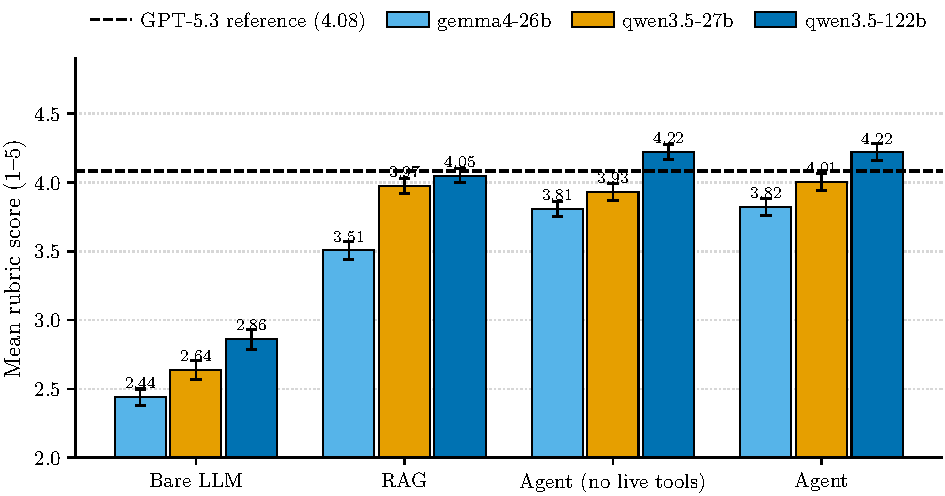
\includegraphics[width=\columnwidth]{figs/fig_headline.pdf}
\caption{The bare LLM, RAG, no-live-tools, and full agent walk
from 2.86 to 4.22 on the largest open-weight model under
\texttt{glm-5.1}; the GPT-5.3 production reference scores 4.08
on the same judge. Mean rubric score per (pipeline,
model), with $\pm 1$ standard error; each cell takes the higher
of the thinking-on/off variants.}
\label{fig:leaderboard}
\end{figure}

\paragraph{(A) An LLM alone fails on CMS-specific facts.}
The bare-LLM band sits at 2.4--2.9 across all three open-weight
models and all six question categories
(Figure~\ref{fig:by_category}). Operator questions target facts
not in pre-training: 76 factual lookups about CMS storage
elements, Rucio rules, and configuration values; 39 Jira
investigations that name specific tickets
(\texttt{CMSPROD-359}, \texttt{CMSTRANSF-1333}, \dots); 34
procedural questions about workflow recovery and resubmission.
A 122\,B model that has not seen the CMS Jira/TWiki/MonIT
corpora at training time cannot answer them; the model emits
plausible-sounding text and the judge penalises it.

\paragraph{(B) RAG closes most of the gap but is blocked on
live state.}
Adding hybrid BM25-plus-vector retrieval over the indexed CMS
TWiki and Jira (the RAG control) lifts the score to
\textbf{3.97}, recovering 1.1 of the 1.4 rubric points lost by
the bare LLM. Indexed documentation is a sufficient source for
the 144 doc-answerable questions, on which RAG averages 3.97
and the full agent 4.10 (Figure~\ref{fig:by_category}). RAG is
structurally blocked, however, on the 116 questions in the
evaluation set that require operational state: a current
transfer rate, a workflow's hourly resubmission count, a site's
readiness flag. The indexed documentation does not contain this
state, and the RAG response on such questions points the
operator to where to look rather than answering the question
directly. On the \textit{data\_query} category specifically,
RAG scores 4.07 and the full agent 4.19, but the rubric is
lenient on look-up-the-runbook responses; the qualitative gap
on live-state questions is wider than the 0.12-point lift the
rubric records.

\paragraph{(C) The agent loop closes the next 0.25 points by
composition.}
The no-live-tools ablation runs the same ReAct loop
as the full agent over the same documentation sources as RAG,
but iterates: search, fetch-by-id, cross-source synthesis. It
reaches \textbf{4.22} against RAG's 3.97 (+0.25), without
adding new tools. The lift is largest on
\textit{jira\_investigation} (4.03 vs 3.87) and
\textit{factual\_lookup} (4.58 vs 4.24): both categories
benefit from composing across multiple retrievals. The same
loop is in the deployed pipeline; the ablation isolates the
contribution of iteration from the contribution of live tools.

\paragraph{(D) Live tools earn their cost only on
data\_query.}
The full agent reaches \textbf{4.22} in aggregate, matching the
no-live-tools ablation at 4.22 because
\textit{data\_query} is 20\% of the dataset. On
\textit{data\_query} alone, live MonIT tools raise the score
from 4.00 to 4.19 (+0.19) by accessing the live counters that
the doc-only configurations cannot reach. On the three
doc-answerable categories (Factual lookup 4.58 vs 4.21;
Procedural 4.30 vs 3.88; Exploratory 4.26 vs 4.16) and on
\textit{jira\_investigation} (4.03 vs 3.70), the no-live-tools
ablation matches or beats the full agent: live calls on
questions whose answer is in the documentation correlate with
lower scores. The mechanism is dilution. Each live MonIT call
returns a JSON payload of operational state that adds hundreds
to thousands of tokens to the agent's context, and the agent
issues several such calls per question
(Section~\ref{sec:eval_costs}, Figure~\ref{fig:tool_usage}). On
a doc-answerable question the additional context crowds out the
retrieved passages that carry the answer, and the judge
penalises the more verbose, less-focused response. The deployed
pipeline keeps live tools enabled because data-query questions
are unanswerable without them; tighter tool-use instructions
that skip live calls when question type does not require them
are a natural next step (Section~\ref{sec:discussion}).

\begin{figure*}[htbp]
\centering
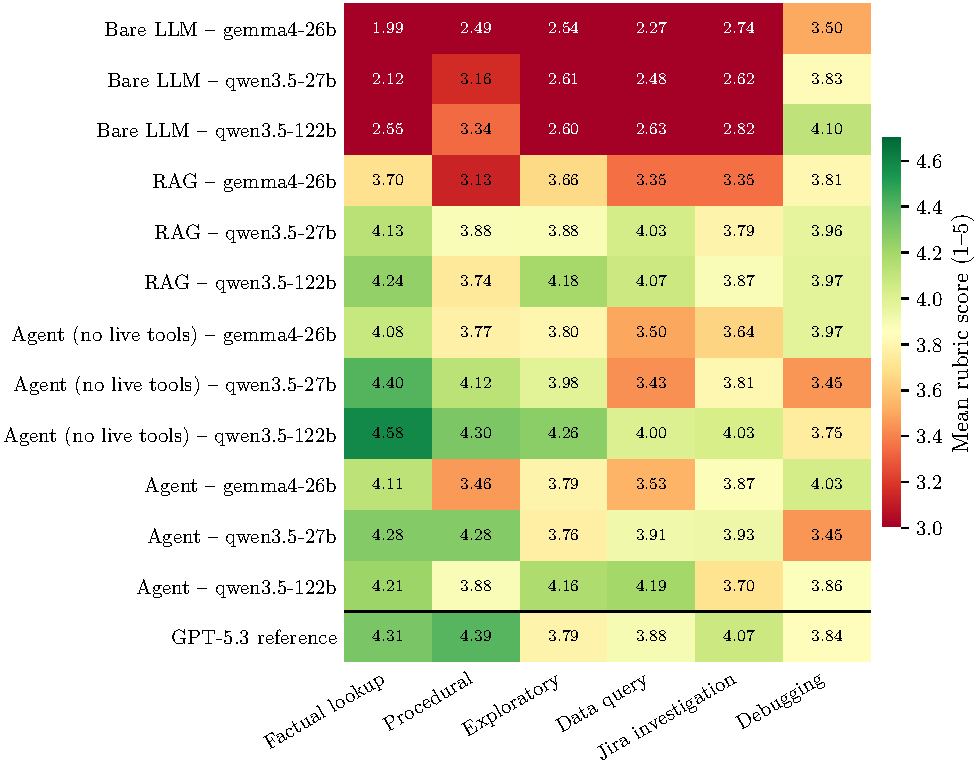
\includegraphics[width=0.82\textwidth]{figs/fig_by_category.pdf}
\caption{Live MonIT tools earn their cost on
\textit{data\_query} and lose 0.05--0.4 points on the three
doc-answerable categories. Mean rubric score per (pipeline,
model), broken down by question category; the bottom row is the
GPT-5.3 reference.}
\label{fig:by_category}
\end{figure*}

The bare-LLM, RAG, no-live-tools, and agent ordering holds on
the smaller two open-weight models as well: on
\texttt{qwen3.5-27b} the agent reaches 4.02 and on
\texttt{gemma4-26b} 3.82. On the largest open-weight model the
agent at 4.22 sits 0.14 points above the GPT-5.3 production
reference at 4.08 under the same judge.

\subsection{Two costs of the agent loop}
\label{sec:eval_costs}

The agent loop closes the gap to the production reference but
carries two measurable costs.

\paragraph{Source-faithfulness inversion.}
Figure~\ref{fig:per_dimension} reports the per-dimension scores
for the \texttt{qwen3.5-122b-a10b} configurations. On the four
core rubric dimensions the agent matches or exceeds the GPT-5.3
reference, with the largest gain on completeness ($+0.3$).
Source faithfulness inverts: the single-shot RAG control scores
\textbf{4.62}, the agent without live tools 3.71, and the full
agent 3.78. The agent's answers cite across many tool returns
rather than a single retrieval pass and score lower on
per-source attribution. The inversion replicates under the
four-judge ensemble of Section~\ref{sec:eval_ensemble}: 4.26
RAG against 3.10--3.74 for the four agents on the 53-question
subset. The same loop that buys composition trades off per-source
attribution.

\begin{figure}[htbp]
\centering
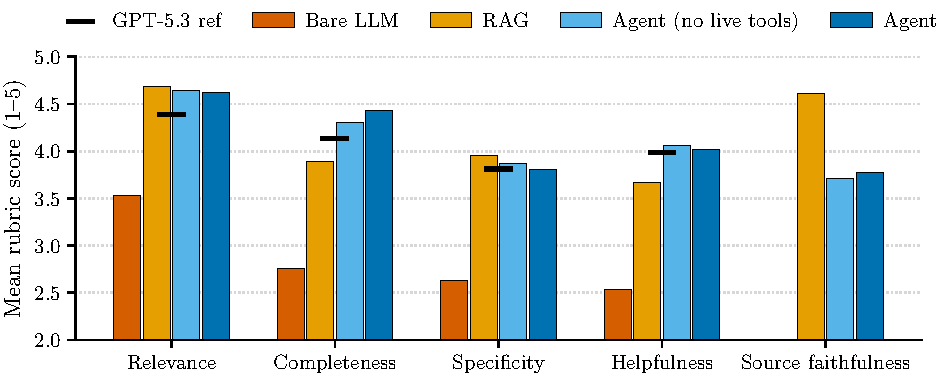
\includegraphics[width=\columnwidth]{figs/fig_per_dimension.pdf}
\caption{The agent matches the GPT-5.3 reference on the four
core dimensions but inverts under source faithfulness, where
the single-shot RAG control (4.62) leads. Per-dimension scores
on \texttt{qwen3.5-122b-a10b}; black ticks mark the GPT-5.3
reference.}
\label{fig:per_dimension}
\end{figure}

\paragraph{Quality--latency tradeoff.}
The agent with live tools runs at 60--150\,s per question on
the largest open-weight model under local Ollama; the RAG
control and the no-live-tools ablation cluster at 13--25\,s on
the same hardware. The full agent is 5--10$\times$ slower
than RAG for an additional 0.0--0.2 rubric points in aggregate.
Table~\ref{tab:runtime_53q} reports the same effect on
OpenRouter, where hosted-inference latency raises the floor.
Extended-thinking variants double the wall time without raising
scores; the deployed assistant runs the agent on the largest
model with extended thinking disabled, keeping operator-facing
latency below 90\,s.

Figure~\ref{fig:tool_usage} shows the agent's tool-call profile
by question category. On \textit{data\_query} the agent issues
5.4 HTCondor MonIT calls per question against 2.3 documentation
calls; on every other category it falls back to documentation
retrieval. The agent self-routes, which is one half of the
routing argument in Section~\ref{sec:discussion}.

\begin{figure}[htbp]
\centering
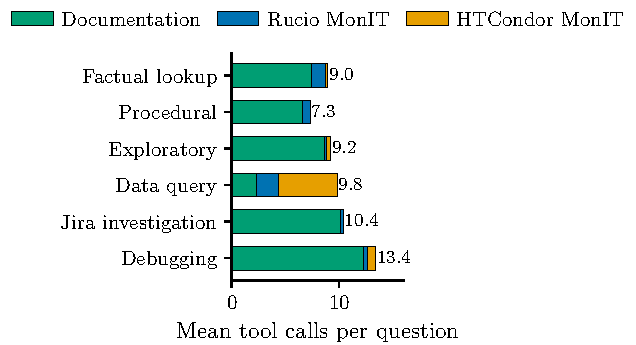
\includegraphics[width=\columnwidth]{figs/fig_tool_usage.pdf}
\caption{The agent routes by question type: HTCondor MonIT
dominates on \textit{data\_query}; every other category falls
back to documentation retrieval. Mean tool calls per question
by category, agent on \texttt{qwen3.5-122b-a10b}.}
\label{fig:tool_usage}
\end{figure}

\subsection{The four-step ordering survives a four-judge ensemble}
\label{sec:eval_ensemble}

Four LLM judges from independent providers rate every response
on the 53-question subset under the rubric of
Section~\ref{sec:eval_methodology}: \texttt{glm-5.1}
\cite{glm130b}, \texttt{gemini-3.1-pro-preview},
\texttt{gpt-5.5-2026-04-23} (rating its own family), and
\texttt{claude-opus-4.7}. All four judges score the 265
(configuration, question) tuples.

Every judge places the closed-frontier \texttt{gpt-5.5}
agent first and the \texttt{qwen3.6-27b} RAG control last
(Table~\ref{tab:judge_ensemble_per_config}). The pipeline
ordering of Section~\ref{sec:eval_lifts} survives a judge swap
on the one configuration shared across both tracks
(\texttt{qwen3.5-122b-a10b} agent) and across four further
configurations the local cluster could not host.

\begin{table*}[htbp]
\centering
\caption{Per-judge per-configuration mean rubric score on the
53-question subset (average of the four core dimensions; 1--5
scale). Every judge places the production-class
\texttt{gpt-5.5} agent first and the \texttt{qwen3.6-27b} RAG
control last.}
\label{tab:judge_ensemble_per_config}
\begin{tabular}{lccccc}
\toprule
\textbf{Configuration} & \textbf{glm-5.1} & \textbf{gemini-3.1-pro} & \textbf{gpt-5.5} & \textbf{opus-4.7} & \textbf{Ensemble} \\
\midrule
\texttt{gpt-5.5-2026-04-23} agent & 4.83 & 4.88 & 4.09 & 4.72 & \textbf{4.63} \\
\texttt{qwen3.6-27b} agent        & 4.56 & 4.83 & 3.71 & 4.49 & \textbf{4.40} \\
\texttt{qwen3.5-122b-a10b} agent  & 4.48 & 4.78 & 3.53 & 4.32 & \textbf{4.28} \\
\texttt{qwen3.6-35b-a3b} agent    & 4.48 & 4.55 & 3.52 & 4.33 & \textbf{4.22} \\
\texttt{qwen3.6-27b} RAG          & 3.95 & 4.41 & 3.26 & 3.50 & \textbf{3.78} \\
\bottomrule
\end{tabular}
\end{table*}

The per-dimension ensemble means
(Table~\ref{tab:judge_ensemble_per_dim}) replicate the
source-faithfulness inversion of
Section~\ref{sec:eval_costs}: the \texttt{qwen3.6-27b} RAG
control scores 4.26 on source faithfulness against 3.10--3.74
for the four agents, while losing 0.5--1.2 points to the
closed-frontier \texttt{gpt-5.5} agent on every other dimension. The
\texttt{gpt-5.5} agent leads on every dimension except source
faithfulness; the open-weight agent ordering is stable across
the four core dimensions.

\begin{table*}[htbp]
\centering
\caption{Per-dimension ensemble-mean rubric score on the
53-question subset (1--5 scale), averaged across the four
judges of Table~\ref{tab:judge_ensemble_per_config}. Source
faithfulness inverts between the agent and RAG pipelines,
matching the 260-question single-judge result of
Section~\ref{sec:eval_costs}.}
\label{tab:judge_ensemble_per_dim}
\begin{tabular}{lccccc}
\toprule
\textbf{Configuration} & \textbf{Relevance} & \textbf{Completeness} & \textbf{Specificity} & \textbf{Helpfulness} & \textbf{Src.\ faith.} \\
\midrule
\texttt{gpt-5.5-2026-04-23} agent & \textbf{4.99} & \textbf{4.79} & \textbf{4.19} & \textbf{4.56} & 3.74 \\
\texttt{qwen3.6-27b} agent        & 4.86 & 4.53 & 3.92 & 4.27 & 3.46 \\
\texttt{qwen3.5-122b-a10b} agent  & 4.82 & 4.48 & 3.72 & 4.10 & 3.25 \\
\texttt{qwen3.6-35b-a3b} agent    & 4.77 & 4.47 & 3.64 & 4.01 & 3.10 \\
\texttt{qwen3.6-27b} RAG          & 4.53 & 3.62 & 3.44 & 3.53 & \textbf{4.26} \\
\bottomrule
\end{tabular}
\end{table*}

One judge-protocol caveat: \texttt{gpt-5.5-2026-04-23} as a
judge is the harshest of the four (4.09 on its own family's
response against the 4.63 ensemble mean) and concentrates that
harshness on the specificity dimension (2.56 against an ensemble
mean of 3.78). The ensemble ordering reported above
de-emphasises this single-judge offset.

\subsection{Human evaluation on the 53-question subset}
\label{sec:eval_human_53}

LLM judges carry length~\cite{hu2025lengthbias},
position~\cite{wang2023fair}, and
self-preference~\cite{panickssery2024selfpref} biases.
A panel of five CMS Computing Operations domain experts grades
the 53-question subset across the five configurations, blind to
configuration, providing a non-LLM reference against which the
judge scores in Sections~\ref{sec:eval_lifts}--\ref{sec:eval_ensemble}
can be checked. The grading round opened on 2026-05-11; results
are reported once the panel completes the round.

The 53 questions are selected by an experienced CompOps operator
from the 260-question curated set of
Section~\ref{sec:question_patterns} and split across
24~factual-lookup, 19~procedural, 5~Jira-investigation,
4~exploratory, and 1~debugging question.
For each question, the five responses are randomly relabeled
A--E with a per-question permutation; the mapping from label to
configuration is hidden from the annotators and stored in a
sidecar. Each response is scored on two 1--5 dimensions:
\emph{correctness} (factual accuracy against operator practice
and the cited sources) and \emph{usefulness} (whether an
on-call operator can act on the response without further
investigation). The annotators also rank A--E from best to
worst, with ties allowed.

The grading platform is Argilla 2.8~\cite{argilla}, deployed on
a CMS-internal node and fronted by an oauth2-proxy GitHub
allowlist. The task-distribution setting requires at least two
submissions per record, so every record carries two or more
independent ratings. Retrieved sources appear as a
metadata-only collapsible block of clickable links (Jira ticket,
TWiki page, GitHub document) rather than as raw retrieved text.

Three quantities are reported once grading completes.
Per-configuration means on correctness and usefulness over the
53 questions place each configuration on the same scale
(Table~\ref{tab:human_eval_per_config}).
Inter-annotator agreement is reported as the mean pairwise
Pearson on the continuous dimensions and mean pairwise
Kendall's~$\tau$ on the rankings, with $r = \textbf{[TBD]}$
and $\tau = \textbf{[TBD]}$. The consistency between the
human ranking and the judge-ensemble ranking from
Section~\ref{sec:eval_ensemble} across the five configurations
is reported as a rank correlation ($\tau = \textbf{[TBD]}$),
bounding how much of the LLM-judge ordering survives under
human scrutiny.

\begin{table*}[htbp]
\centering
\caption{Per-configuration human-evaluation results on the
53-question subset, averaged across the annotator panel.
Correctness and usefulness are 1--5 means; rank is the mean
A--E ranking position (1 = best). Values pending the close of
the grading round.}
\label{tab:human_eval_per_config}
\begin{tabular}{lccc}
\toprule
\textbf{Configuration} & \textbf{Correctness} & \textbf{Usefulness} & \textbf{Mean rank} \\
\midrule
\texttt{gpt-5.5-2026-04-23} agent & \textbf{[TBD]} & \textbf{[TBD]} & \textbf{[TBD]} \\
\texttt{qwen3.5-122b-a10b} agent  & \textbf{[TBD]} & \textbf{[TBD]} & \textbf{[TBD]} \\
\texttt{qwen3.6-35b-a3b} agent    & \textbf{[TBD]} & \textbf{[TBD]} & \textbf{[TBD]} \\
\texttt{qwen3.6-27b} agent        & \textbf{[TBD]} & \textbf{[TBD]} & \textbf{[TBD]} \\
\texttt{qwen3.6-27b} RAG          & \textbf{[TBD]} & \textbf{[TBD]} & \textbf{[TBD]} \\
\bottomrule
\end{tabular}
\end{table*}

\section{Discussion}
\label{sec:discussion}

\paragraph{Comparison to alternatives.}
A documentation-only retrieval chatbot~\cite{lewis2020rag} cannot
answer the 116 live-state questions in the evaluation set
(counters such as a transfer rate, a workflow's resubmission
count, or a site's hourly readiness flag) because the indexed
documentation does not contain operational state. A single tool
call~\cite{yao2023react} reaches MonIT but does not compose
across sources: triaging a stalled transfer requires the runbook
entry, the current site-readiness counter, and the ticket history
of past stalls on the same link, and the iterative ReAct loop is
what threads them together. AccGPT~\cite{accgpt2025} and
chATLAS~\cite{chatlas2025} deploy retrieval-augmented assistants
over CERN- and ATLAS-wide documentation but do not pair retrieval
with live operational tool calls or report a rubric-based
evaluation against a curated production-question dataset.
GAIA~\cite{mayet2024gaia} pairs ReAct over an open-weights LLM
with control-system tools and a multi-expert RAG layer at DESY,
and the multi-lab logbook work~\cite{sulc2024logbooks} extracts
insight from electronic logbook entries at DESY, BESSY, Fermilab,
BNL, SLAC, LBNL, and CERN; both target accelerator operations
rather than offline computing operations and do not evaluate
against a curated production-question dataset.

\paragraph{Bounding the live-tool cost.}
The full agent and the no-live-tools ablation tie in aggregate
because live tools help on the 20\% of operator traffic that
needs operational state and dilute the context on the other
80\% (Section~\ref{sec:eval_lifts}). The dilution is mechanical:
each live MonIT return is a structured payload of hundreds to
thousands of tokens, and the agent issues several per question.
The path to recover the per-category gap is not a separate
upstream classifier but tighter tool-use instructions inside the
agent itself: condition the decision to call MonIT on a
short, structured judgement about whether the question requires
operational state, and skip the live calls when the answer is
already in the documentation. The agent already self-routes its
tool families by question type
(Figure~\ref{fig:tool_usage}); the remaining lift is making the
``call no live tool'' branch first-class.

\paragraph{The source-faithfulness inversion.}
The agent's multi-pass reasoning trades single-passage citation
for cross-source synthesis. On the 260-question single-judge run
the agent scores 3.78 on source faithfulness against the RAG
control's 4.62; the same inversion replicates on the
53-question four-judge ensemble (3.10--3.74 for the agents
against 4.26 for the RAG control). The deployed UI exposes the
agent's tool-call trace per response as partial mitigation:
operators can audit which retrieval each claim came from even
when the rubric scores the cross-source synthesis lower on
attribution. A knowledge-graph-backed retrieval layer is the
deeper fix; we sketch it below.

\paragraph{Judge methodology.}
The reference-free rubric reduces some dependence on the judge,
but the per-pipeline scores and the source-faithfulness inversion
inherit known LLM-judge biases. The four-judge LLM ensemble on
the 53-question subset (Section~\ref{sec:eval_ensemble}) agrees
with the single-judge ordering across independent providers; the
harshest judge, \texttt{gpt-5.5}, diverges most on specificity.
The human evaluation of Section~\ref{sec:eval_human_53} provides
the non-LLM reference once it completes.

\paragraph{Richer knowledge representation.}
The retrieval layer is currently a hybrid BM25-plus-vector index
over passages (Section~\ref{sec:components}), and the agent's
live-tool surface covers Rucio MonIT and HTCondor MonIT only.
Operator workflows also touch Oracle-backed services and Indico,
which are part of the deployment but not yet exposed as agent
tools. We are designing a knowledge-graph-backed retrieval layer
that exposes ticket--site--workflow--dataset relations directly,
distinguishes stale fields (last-known transfer state) from
durable metadata (site endpoints, dataset lineage), and lets
the agent traverse paths that passage retrieval cannot. The same
layer plugs in additional live sources without re-architecting
the pipeline.

\section{Conclusions and Outlook}
\label{sec:conclusions}

Archi has run as the CMS Computing Operations operator chat
assistant since February 2026, pairing hybrid retrieval over the
CMS TWiki and Jira with live MonIT queries against Rucio and
HTCondor in a ReAct loop. On a 260-question evaluation set
sampled from six weeks of production operator traffic, the four
pipeline layers (bare LLM, RAG, agent without live tools, full
agent) walk from 2.86 to 4.22 on the rubric under
\texttt{glm-5.1} on the largest open-weight model; each layer
earns its keep, and the full agent at 4.22 lands 0.14 points
above the GPT-5.3 production reference (4.08) on the same
judge. A four-judge LLM ensemble on a 53-question subset
(Section~\ref{sec:eval_ensemble}) preserves the pipeline
ordering, and a parallel human evaluation by a CompOps domain
expert panel (Section~\ref{sec:eval_human_53}) provides the
non-LLM cross-check once it completes. The next architecture step is a knowledge-graph-backed
retrieval layer that exposes ticket--site--workflow--dataset
relations directly and narrows the source-faithfulness gap
between the agent loop and single-shot RAG.


% Acknowledgements heading restored when content lands.
% TODO: Acknowledgements paragraph. Standard CHEP form: CMS Collaboration,
% CERN, MIT SubMIT, named operators who provided feedback during deployment,
% and funding agencies per co-author affiliations.

% bibliography style is set by webofc (woc.bst).
\bibliography{refs}

\end{document}
